% !TEX encoding = UTF-8
% !TEX TS-program = pdflatex
% !TEX root = ../tesi.tex
% !TEX spellcheck = it-IT

%**************************************************************
\chapter{Valutazione Retrospettiva}
\label{cap:valutazione-retrospettiva}
%**************************************************************
\intro{Questo capitolo riporta un bilancio finale su quanto svolto durante lo stage.}




%**************************************************************************************************
\section{Bilancio sui risultati}
In questa sezione riassumo gli obiettivi aziendali e gli obiettivi personali raggiunti durante lo stage.
\subsection{Obiettivi conseguiti}
Gli obiettivi fissati all'inizio dello stage hanno subito delle modifiche perché l'azienda ha voluto privilegiare il porting di DRE. Il \emph{porting} dell'applicativo è parzialmente completato, l'unica funzionalità non ancora implementata una procedura di \emph{map-reduce}. Quest'ultima funzionalità non l'ho completata perché implementata con la tecnologia javascript da eseguire all'interno di MongoDb, le mie competenze per comprendere quel codice erano insufficienti ed avrebbero introdotto un ulteriore ritardo per lo sviluppo di Tres inoltre l'obiettivo di migliorare la fase di apprendimento di questo modulo non l'ho raggiunto. Durante lo sviluppo di Tres ho individuato 23 requisiti di cui 20 obbligatori e 3 desiderabili.  
\begin{figure}[h]
\centering
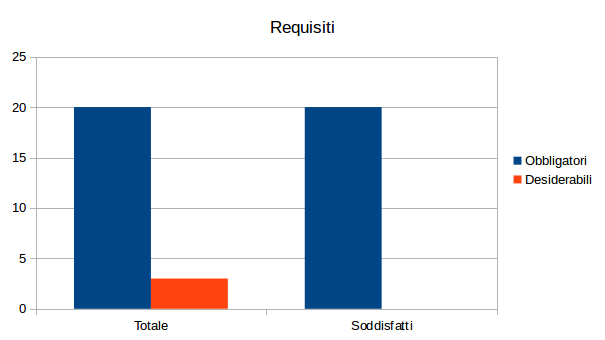
\includegraphics[scale=0.62]{immagini/graficorequisiti}
\caption{Riassunto requisiti}
\label{fig:client-server}
\end{figure}
\\I requisiti non soddisfatti riguardano direttamente gli obiettivi (e quindi non ho raggiunto) di implementazione di algoritmi di \emph{clustering} e di implementazione di algoritmi per l'individuazione dei gusti dell'utente. Tuttavia quest'ultimo obbiettivo l'ho centrato grazie all'implementazione di ID3 per fornire una raccomandazione sulla base del comportamento utente. Infine in questa attività ho soddisfatto l'obbiettivo minimo riguardante l'utilizzo di OrientDb.
\subsection{Obiettivi personali}
All'inizio dello stage il mio obbiettivo era quello di imparare nuove tecnologie da aggiungere alle mie conoscenze perché ritenevo il mio bagaglio personale insufficiente per affrontare il mondo del lavoro. Questo obbiettivo è stato certamente raggiunto, infatti lo stage mi ha permesso di padroneggiare ad un buon livello tecnologie quali OrientDb, web framework di concezione moderna e Scala. Quest'ultimo mi ha dato la possibilità di apprendere le nozioni per un corretto stile di programmazione funzionale, che era uno degli obbiettivi prefissatomi. Ritengo l'obbiettivo riguardante l'approfondimento di argomenti quali, intelligenza artificiale e i sistemi di raccomandazione, parzialmente soddisfatto. Durante lo stage non ho trovato il supporto necessario per approfondire queste competenze, soprattutto per quanto riguarda i sistemi di raccomandazione visto la natura del progetto di stage.
%**************************************************************************************************




%**************************************************************************************************
\section{Bilancio formativo}
In questa sezione viene riportato le competenze acquisite durante lo stage.\\
Lo stage in Nextep Srl è stata la  mia prima esperienza nel settore informatico, mi ha permesso di apprendere nuove competenze e consolidare competenze già apprese durante il corso di studi.
%Prima avevo idee molto confuse a riguardo la mia carriera professionale, ma ora dopo lo stage posso affermare di avere aspettative più ambiziose e idee più chiare su quale cammino professionale intraprendere.
Ho trovato molto positivo lavorare collaborativamente al progetto perché questo mi ha portato ad migliorare le mie capacità di \emph{team working}, una \emph{skill} molto importante nel mondo del lavoro soprattutto nei contesti lavorativi dove si utilizza una metodologie \emph{agile}. Ho migliorato le mie capacità di \emph{project management} per concludere il progetto nei tempi fissati e raggiungere gli obbiettivi minimi che mi sono prefissato. In conclusione ho concluso lo stage con un bagaglio professionale più ricco e di essere in grado di farmi carico di responsabilità più importanti.
\subsubsection{Scala}
Durante lo stage ho avuto modo di apprezzare i vantaggi derivanti dall'uso di questo linguaggio. Ho utilizzato questa tecnologia nelle attività di \emph{porting} del modulo DRE e nell'attività di sviluppo di Tres. Per studiare Scala ho seguito un corso \emph{online}\footcite{https://www.coursera.org/course/progfun} tenuto direttamente dal professore Martin Odersky\footcite{http://lampwww.epfl.ch/~odersky/}, ovvero il \emph{designer} del linguaggio stesso. Un corso validissimo per capirne i meccanismi e le peculiarità di questo linguaggio. All'inizio è stato un po' ostico mettere in pratica quanto appreso, ma quando ho cominciato a padroneggiare Scala ho potuto constatare un aumento della mia produttività. Ho trovato un po' macchinoso gestire la compatibilità con librerie Java di terze parti. Mi ritengo soddisfatto di aver imparato questa tecnologia e di poter reinvestire nel mondo del lavoro questa conoscenza. 
\subsubsection{Programmazione funzionale}
La competenza più importante che ho acquisito durante lo \emph{stage} è stato il paradigma di programmazione funzionale. Questo paradigma mi ha fornito una modalità diversa di affrontare e risolvere problemi rispetto alla classica programmazione orientata agli oggetti. Nella programmazione funzionale vengono evitati i dati di stato e modificabili e viene data invece una maggiore enfasi all'applicazione di funzioni. Mantenere gli stati immutabili facilita la suddivisone del codice per l'esecuzione parallela garantendone la correttezza, questa caratteristica è importantissima al giorno d'oggi dove il focus si sta via via spostando sempre di più verso contesti multi-threading. %Per concludere questo paradigma induce ad uno stile di programmazione più espressivo e conciso 
\subsubsection{OrientDb}
Questa tecnologia è la soluzione di persistenza adottata durante il progetto. La curva di apprendimento è stata molto rapida, grazie al corso online\footcite{https://www.udemy.com/orientdb-getting-started/} tenuto durante l'attività di formazione. Mi ha permesso di imparare le differenze tra i modelli più tradizionali come i relazionali e i modelli a grafo. Le modelli a grafo si prestano molto bene per soluzioni nel dominio web soprattutto in questo momento storico che il web si sta evolvendo in web semantico. E' stato un po' difficoltoso all'inizio passare dal concetto di \emph{Join} delle tabelle al concetto \emph{Traverse} dei grafi. Tuttavia la modellazione del dominio con un grafo è stata molto più semplice ed intuitiva rispetto ad un modello relazionale. 
\subsubsection{Play Framework}
L'apprendimento di questo \emph{framework} non è particolarmente difficile, perché la documentazione presente nel sito è molto esaustiva e fornisce supporto completo per la configurazione di una web application. Trovo molto vantaggioso la compatibilità con i linguaggi Java e Scala in modo da poter sviluppare una applicazione con entrambi i linguaggi. La prima configurazione iniziale è stata molto semplice, questo mi ha permesso di focalizzarmi subito allo sviluppo del modulo. Purtroppo ho trovato complicato testare parti del mio modulo perché era necessario per il test avere l'istanza del server avviata. Si integra bene con scala...
%**************************************************************************************************




%**************************************************************************************************
\section{Distanza tra formazione universitaria e lavoro}
In questa sezione sezione viene esposto la valutazione personale della distanza tra la formazione ricevuta durante il corso di studi e lo stage formativo.
Questa esperienza mi ha permesso di valutare la distanza tra la formazione universitaria e le competente realmente richiesta durante lo stage.
La prima difficoltà che ho incontrato riguarda l'attività di modellazione del database. Mi sarebbe stato utile avere delle nozioni per affrontare una modellazione su di un database a grafo, invece durante il corso di \emph{Basi di Dati} vengono insegnate solamente soluzioni di database relazionali. Sarebbe sufficiente introdurre dei fondamenti sulle varie tipologie di database in modo che lo studente possa valutare pro e contro di ogni tipologia e utilizzare la soluzione migliore a seconda del contesto.

%Trovo molto grave che nel corso di \emph{Tecnologie Web} non sia neppure menzionata la tecnologia \emph{REST}. Nel dominio \emph{web} questa tecnologia ha già assunto una importanza tale da meritare un approfondimento per evitare che si diffondano implementazioni non aderenti allo standard. (RIVEDERE)



%L'insegnamento che mi ha maggiormente preparato per questa esperienza è sicuramente \emph{Ingegneria Del Software}. Grazie a questo corso ho appreso molte nozioni tecniche e un approccio valido per la gestione e la produzione software, un bagaglio molto importante più che sufficiente per i progetti futuri.
%Ritengo che durante il corso di laurea sia dato poco spazio per apprendere tecniche di programmazione valide ed evitare quindi errori comuni (spesso perché si fa affidamento a corsi online), sarebbe utile potenziare il corso di \emph{programmazione ad oggetti} introducendo alla fine del programma i design pattern e come utilizzarli efficacemente. Magari se non nel corso di \emph{Programmazione}, ritengo importante spiegare come utilizzare sapientemente strumenti per fare il testing del codice, e i debugger per individuare errori nel codice.

Il corso di laurea mi ha fornito le nozioni fondamentali per poter affrontare egregiamente il lavoro, proprio per questo motivo durante lo stage non mi sono mai trovato davanti a delle difficoltà che ostacolassero le attività assegnatomi.
%**************************************************************************************************